\documentclass[a4paper,twoside]{IEEEtran}

\newcommand{\seminarteilnehmer}{Tim Budweg}
\newcommand{\seminartitel}{TODO: Der Titel Ihrer Seminararbeit}

% Löschen oder kommentieren Sie die folgenden beiden Zeilen aus,
% wenn Sie den Text in Englisch schreiben wollen.
\usepackage{german}
\usepackage[utf8]{inputenc}

\usepackage{graphicx}
\graphicspath{{figures/eps/}}
\usepackage{ dsfont }




\usepackage{amsmath}


\begin{document}

\title{\seminartitel}
\author{\seminarteilnehmer}

\markboth{Seminar Rechnernetze, Wintersemester 2014/2015}%
{\seminarteilnehmer: \seminartitel}


\maketitle

\begin{abstract}
TODO: Die Zusammenfassung zu Ihrer Seminarausarbeitung.
\end{abstract}

\begin{IEEEkeywords}
TODO: Stichworte zu Ihrem Seminarthema.
\end{IEEEkeywords}


\section{Einleitung}
Es gibt viele Anwendungsbereiche für drahtlose Sensornetze. 
Zum Beispiel können Waldbrände oder Tsunamis durch ein Frühwarnsystem, welches durch ein Sensornetz realisiert wird, schneller erkannt werden. 
Sowohl in diesem Beispiel als auch in anderen Anwendungsgebieten ist es gewünscht, dass alle gesendeten Nachrichten ankommen.
Garantierte Nachrichtenauslieferung wird von mehreren Algorithmen bereits erreicht (z.B.: Face-Routing: siehe \cite{FaceRouting}).
Jedoch müssen dafür bestimmte Voraussetzungen an das Sensornetz erfüllt sein. 
Die wichtigste Voraussetzung ist die Planarität des Netzes, das heißt, dass keine Kantenschnitte existieren dürfen. 
Diese Planarität zu erreichen ist ein wichtiges Ziel von \textit{Topologiekontrollen}.

Ein weiterer Punkt ist, dass diese Netze willkürlich groß werden können.
Deshalb führt ein \textit{zentralisierter} Algorithmus zu einer sehr langen Laufzeit mit hohem Energieverbrauch, weil Nachrichten in Abhängigkeit von der globalen Netzgröße verschickt werden müssen. 

Damit die Nachrichten nicht über beliebig lange Pfade geroutet werden müssen, wird eine Beschränkung der Pfadverlängerung gewünscht. Pfadverlängerungen entstehen, wenn (spezielle) kantenlöschende Algorithmen auf Graphen angewendet werden.
Der hier behandelte Algorithmus ist streng lokal, was die Anzahl der gesendeten Nachrichten minimiert.
Außerdem produziert dieser einen \textit{t-Spanner} des euklidischen Graphen.
%\textit{t-Spanner} geben den größtmöglichen Umweg an, der entsteht, wenn man einen (speziellen) kantenlöschenden Algorithmus auf einen Graphen anwendet.
Diese Thematik wird im Folgenden anhand des Artikel von \cite{kanj} erläutert.
Dort wurde ein streng lokaler Algorithmus aufbauend auf den \textit{Delaunay Graphen} angewandt.
Das Ergebnis ist ein Graph, welcher im Bezug zum euklidischen Graphen einen \textit{stretch-factor} von $t=3.54 $ und zusätzlich eine Beschränkung des Ausgangsgrad eines Knoten von $k=14 $ hat.



%Spanner?


%\subsection{Planarität}
%Ein Graph ist planar, wenn es keine zwei Kanten gibt, die sich schneiden.

\subsection{Graphen}
\subsubsection{Euklidischer Graph}
Ein euklidischer Graph ist ein spezieller Graph. Alle Knoten sind mit allen anderen Knoten verbunden (Clique) und die Kantengewichte entsprechen der euklidischen Distanz beider Eckpunkte. Ein Beispiel finden Sie in Abbildung \ref{fig:Graph}.
\begin{figure}[h!]
\centering

\includegraphics[width=0.99\linewidth]{Graph.eps}
\caption{Ein euklidischer Graph}
\label{fig:Graph}
\end{figure}
\subsubsection{Unit Disk Graph}
Der Unit Disk Graph ist ein euklidischer Graph ohne alle Kanten, die länger als ein konstantes $c \in \mathds{R} $ sind. In Abbildung \ref{fig:UnitGraph} sehen Sie den euklidischen Graph aus Abbildung \ref{fig:Graph} als Unit Disk Graph mit $c = 1 $.
\begin{figure}[h!]
\centering
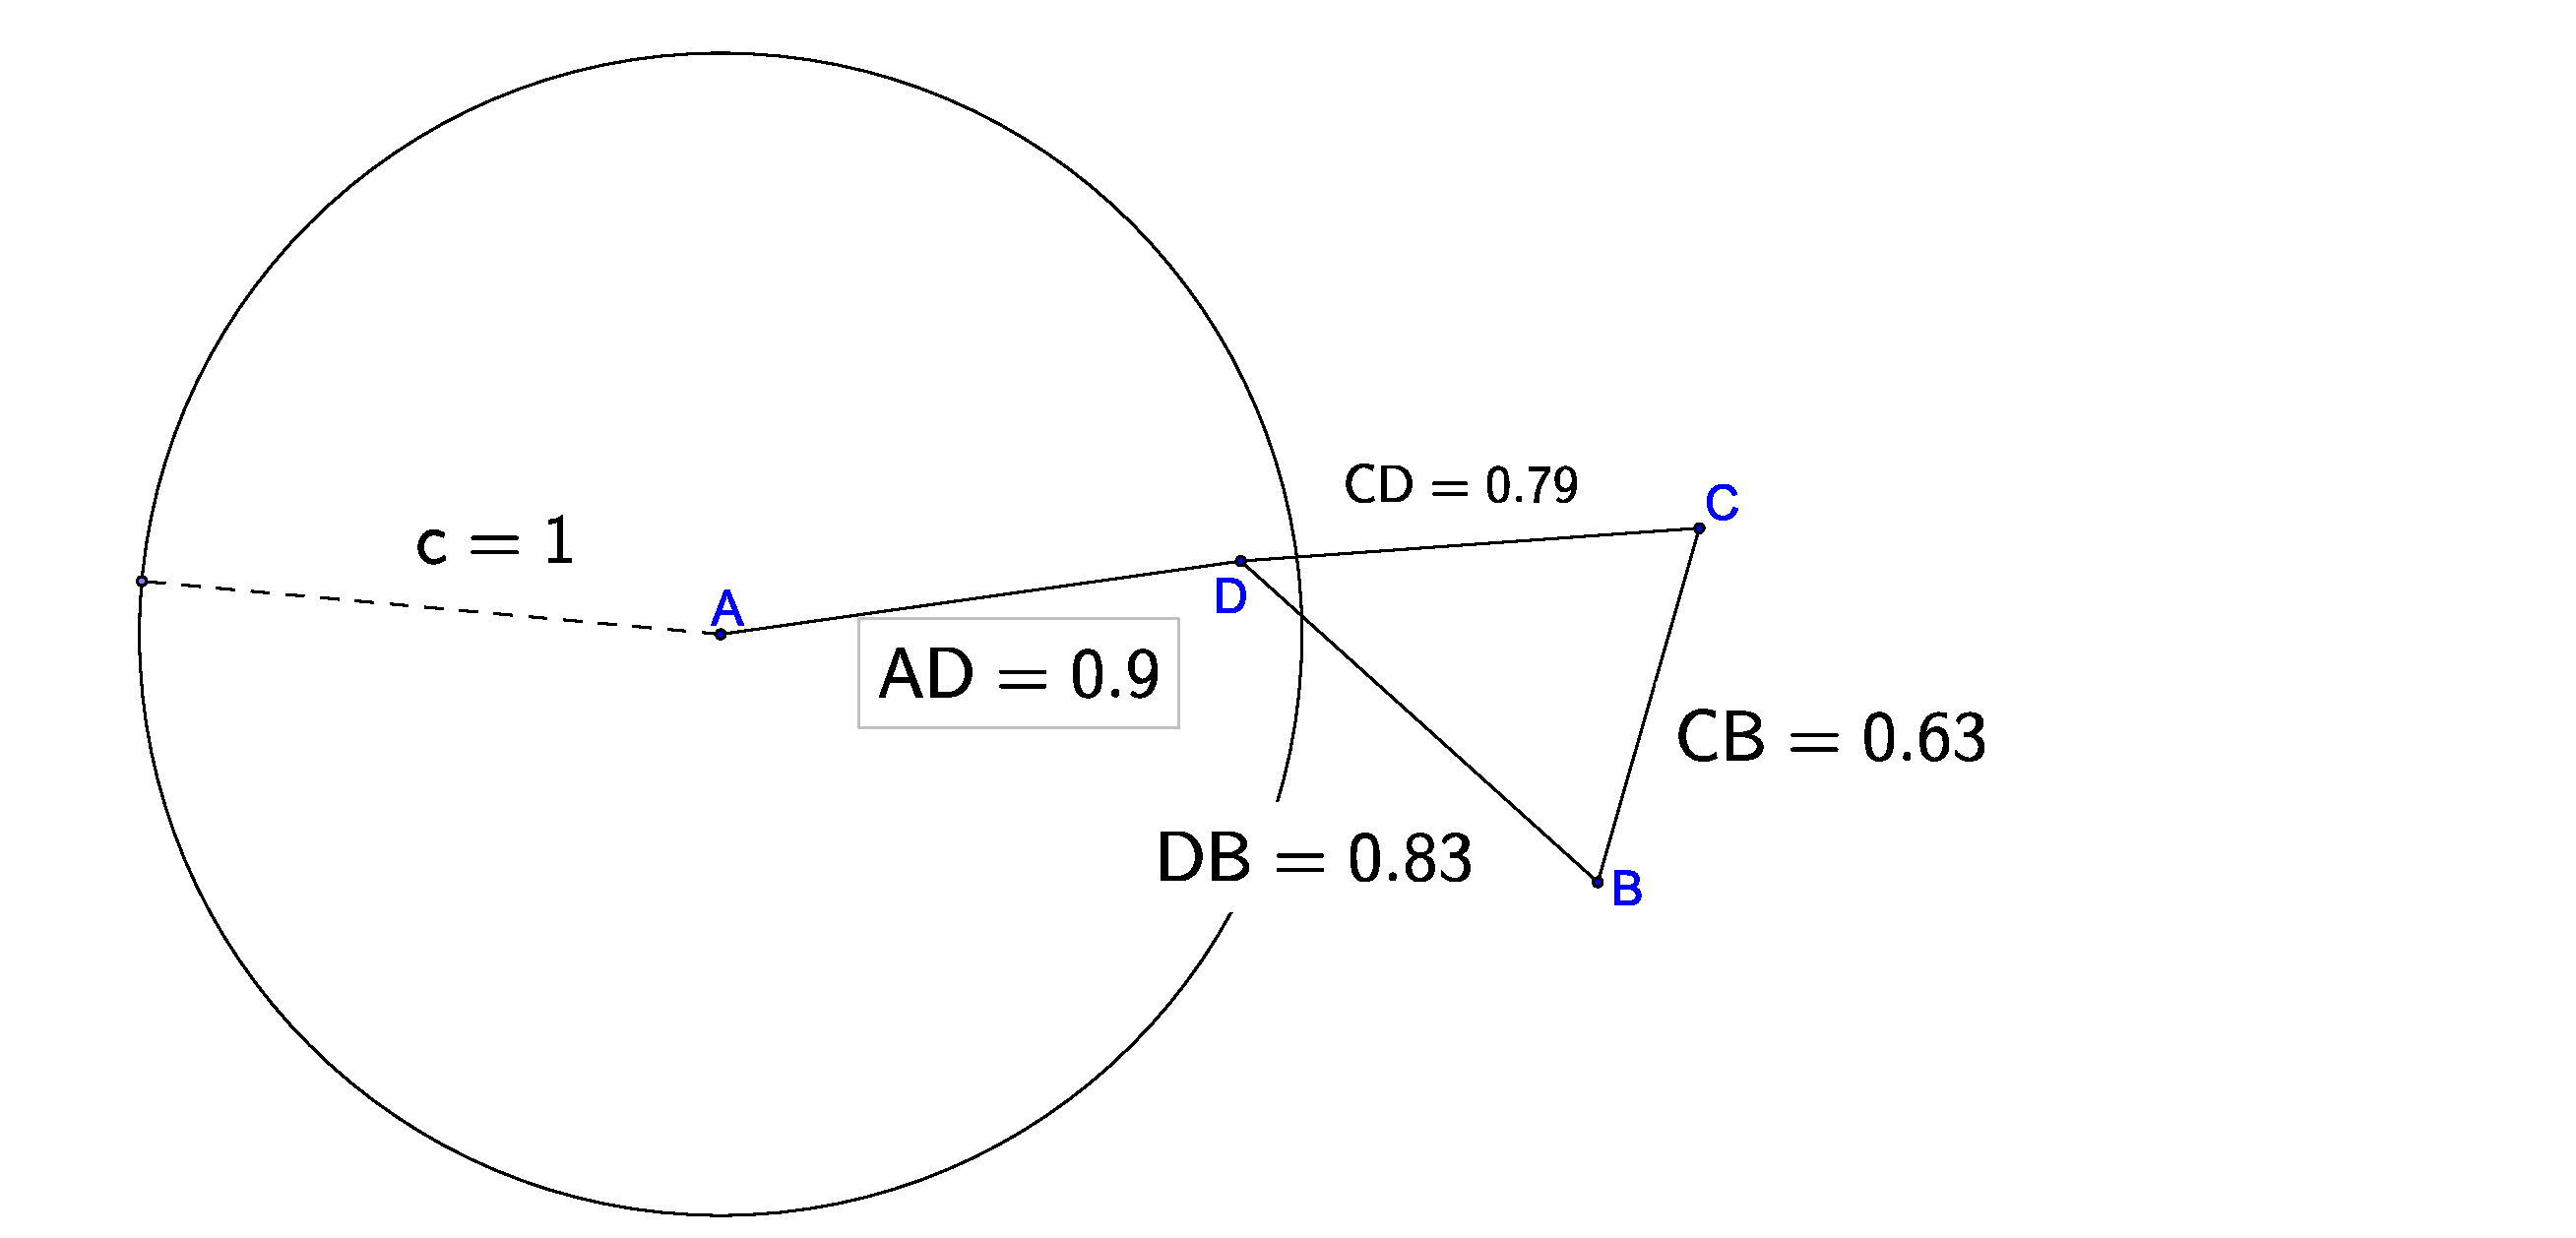
\includegraphics[width=0.99\linewidth]{UnitGraph.eps}
\caption{Der Unit-Disk-Graph zu Abbildung \ref{fig:Graph} mit $c = 1 $}
\label{fig:UnitGraph}
\end{figure}



\subsection{Spanner}
Gegeben ist ein Graph $G $, welcher ein Subgraph vom euklidischen Graphen $E $ ist. $G $ enthält alle Knoten von $E $, aber nicht alle Kanten. Die Umwege, die durch das Löschen von Kanten entstehen, dürfen nur um einen konstanten Faktor ansteigen. 

\subsubsection{Euklidischer Spanner}
$G $ ist genau dann ein euklidischer Spanner von $H $, wenn die kürzesten Pfade zwischen allen Knoten maximal um einen konstanten Faktor $t $ vergrößert werden.
Die Notation $c_{G}(A, B) $ bedeutet: der kürzeste Pfad zwischen A und B im Graphen $G $.
Formal bedeutet das:
\begin{equation}
	c_H(A, B) \leq p \cdot c_G(A, B)
\end{equation}
{\footnotesize (Formel entnommen aus \cite{kanj})}

\subsection{Yao Step}
Gegeben ist ein Graph $G $. Für alle Knoten $A \in G $ wird folgender Algorithmus ausgeführt:
\begin{enumerate}
\item Erzeuge k gleich große Kegel um $A $. $k \in \mathds{N} > 6 $
\item Bestimme die kürzeste Kante in jedem Kegel ausgehend von $A $.
\item Lösche alle Kanten, die nicht von beiden Endpunkten ausgewählt wurden.

\end{enumerate} 
%Dadurch entsteht Graph $G' $. 

\subsection{Delaunay Triangulation}
Die Delaunay Triangulation erzeugt aus einem beliebigen zusammenhängenden Graphen einen geometrischen (= euklidischen) Spanner mit dem Streckungsfaktor $c_{del} \approx 2.42 $ und einem beliebig hohen Ausgangsgrad eines Knotens. 
Dazu werden alle Dreiecke betrachtet.
Wenn der Kreis durch alle Eckpunkte des Dreiecks keine weiteren Punkte des Graphen enthält, sind diese drei Kanten auch im Delaunay Graphen. 
Um Fallunterscheidungen zu vermeiden wird angenommen, dass keine vier Punkte auf einem Kreis liegen. 


\subsubsection{Synchronität}
Bei einem synchronen Algorithmus ist die Arbeitsweise der Knoten in Runden und diese in Phasen eingeteilt. 
Eine Runde sieht beispielsweise wie folgt aus:
\begin{enumerate}
\item Zuerst erhalten alle Knoten ihre Nachrichten, falls es welche gibt.
\item Danach verarbeiten sie die Nachrichten und stellen ggf. weitere Berechnungen an.
\item Am Ende der Runde werden Nachrichten an andere Knoten verschickt.
\end{enumerate}
Hier ist zu beachten, dass alle gesendeten Nachrichten \textbf{nur} zu Beginn der Folgerunde ankommen.

%Algorithmus, definieren, dass es sich hier um Algorithmen auf Graphen handelt?
\subsection{Lokale Algorithmen} \label{lokal}
Ein Algorithmus ist genau dann lokal, wenn jeder Knoten ausschließlich mit seiner \textit{k-Hop} Nachbarschaft kommuniziert. ($k \in \mathds{N}$)
Formal reicht dies aus, um einen Algorithmus lokal zu nennen.
Das Problem, dass der Algorithmus eine lange Laufzeit hat (siehe Einleitung), ist dadurch jedoch nicht gelöst.
Anhand des \textit{Maximal Independent Set} Algorithmus lässt sich ein Beispiel konstruieren, welches dieses Problem veranschaulicht.
%Es soll das \textit{Maximal Independent Set} (MIS) eines Graphen $G $ berechnet werden.
Betrachten Sie Abbildung \ref{fig:MIS}.

\begin{figure}[h!]
\centering
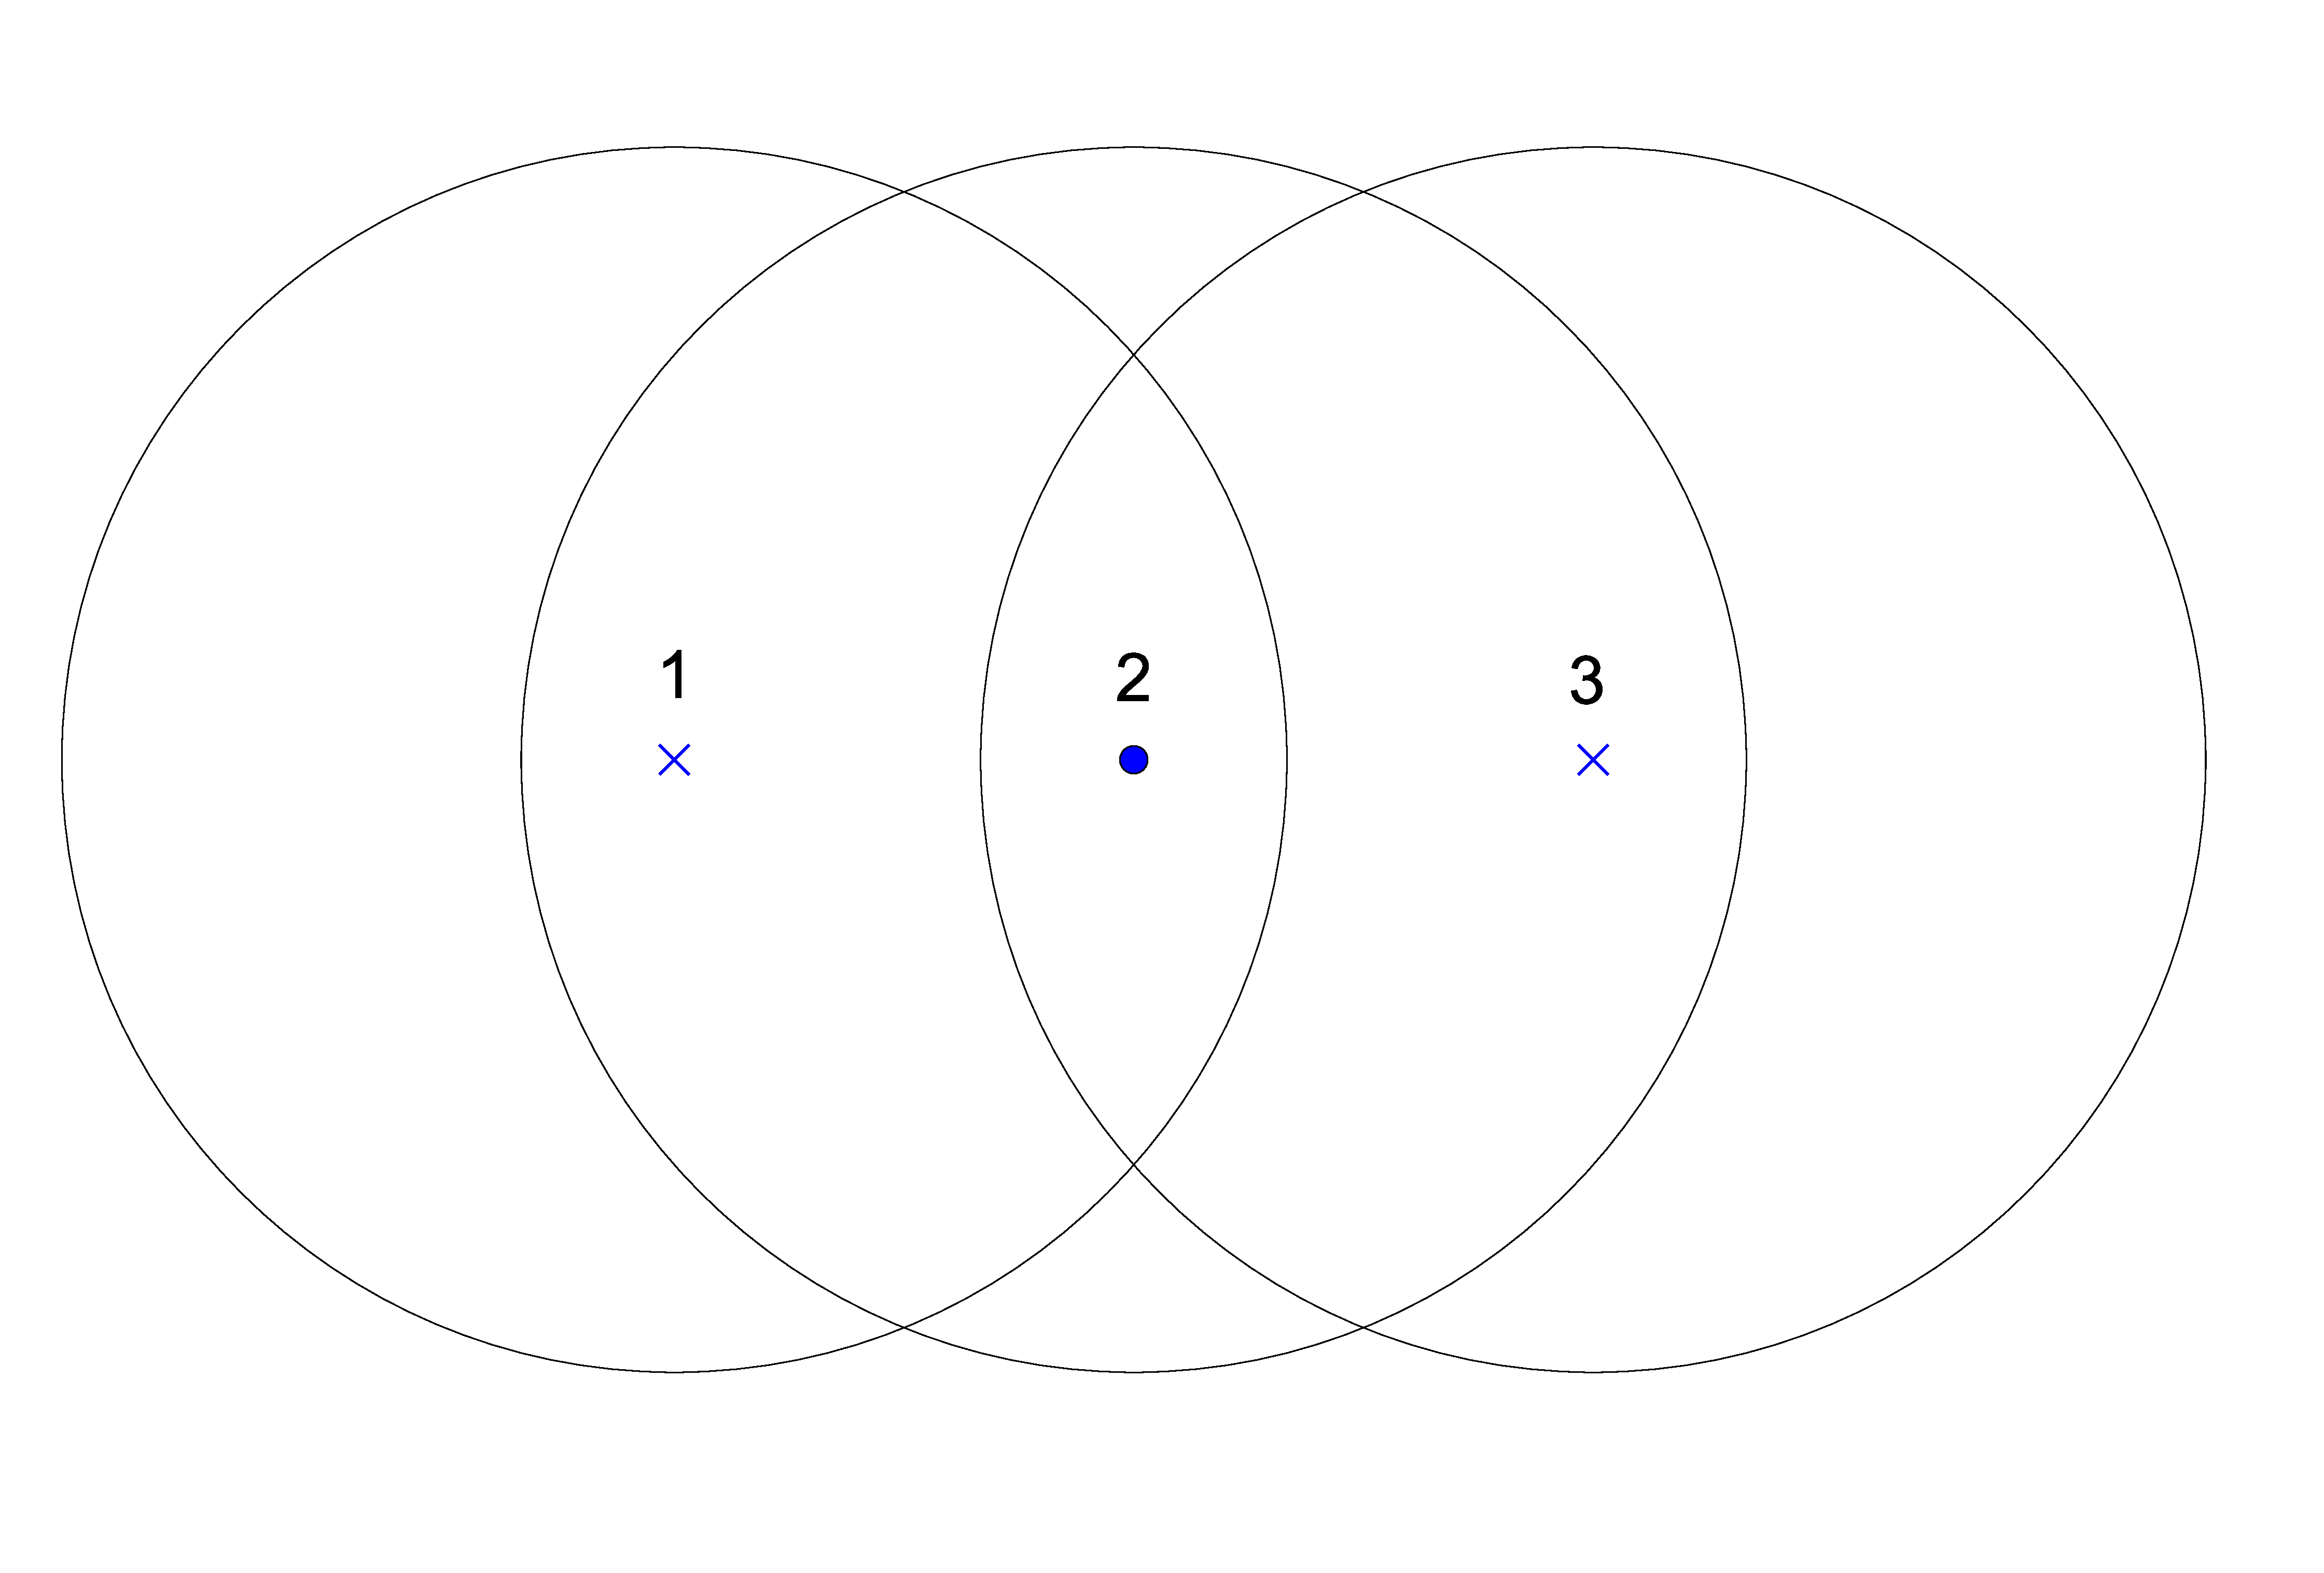
\includegraphics[width=0.99\linewidth]{MIS.eps}
\caption{$\times $ sind Knoten im Maximal Independent Set (Fortan: MIS), $\bullet $ sind keine Knoten des MIS, Die Kreise um die Knoten sind die jeweiligen Sendebereiche.}
\label{fig:MIS}
\end{figure}


\begin{enumerate}
\item[Runde 1] Knoten 1 wird MIS-Knoten, da er von allen seinen Nachbarn, welche noch keine Rolle haben, derjenige mit der kleinsten ID ist. Knoten 2 und 3 warten, da es Knoten gibt, welche noch keine Rolle und eine kleinere ID haben.

\item[Runde 2] Knoten 2 entscheidet, dass er kein MIS-Knoten ist, da er in seiner Nachbarschaft Knoten 1 kennt, der schon MIS-Knoten ist. Knoten 3 wartet.

\item[Runde 3] Knoten 3 wird MIS-Knoten, da Knoten 2 kein MIS-Knoten ist und somit 3 die kleinste ID hat. 

\end{enumerate}

Diese Schritte lassen sich durch den gesamten Graphen sukzessiv durchführen. 
Der Algorithmus hat demnach eine Laufzeit in der Größenordnung von 
\begin{equation*}
\theta (dia(G)) 
\end{equation*}
wobei $dia(G) $ für den Durchmesser (größter kürzester Pfad) des Graphen steht.

Die Definition des lokalen Algorithmus trifft hier zu, weil jeder Knoten nur mit seinen unmittelbaren Nachbarn, der \textit{1-Hop-Nachbarschaft}, kommuniziert.





\subsection{Strenge Lokalität}
Wie im Abschnitt \ref{lokal} beschrieben, sind lokale Algorithmen noch nicht ausreichend, um die benötigte Nachrichtenanzahl zu minimieren.
Ein Algorithmus ist genau dann streng lokal, wenn er unabhängig von der Netzgröße in konstanter Zeit terminiert (siehe \cite{strictlyLocal}).


\subsubsection{title}


\section{was erreicht diese Arbeit} %bearbeiten

\section{Geometrische Spanner}
\subsection{Der outward Path}
\subsection{Der inward Path}


\section{Fazit}



\bibliographystyle{IEEEtran}
\bibliography{biblio}


\end{document}
